\section{Audiosense Design}
\subsection{Field Study}
In this \cite{hasan:PH14}
\subsection{Software Implementation}
\subsection{Calibration}
\subsubsection{Frequency Response}
Frequency response tests help us in understanding the underlying characteristics of the mobile phone's microphone. We ran a series of response tests within the frequency band of 1000Hz -- 6000Hz, covering frequencies in which human speech lies. The input signal was varied from 50dB in steps of 5dB until the amplitude reached 80dB. As it can be seen in Figure \ref{fig:calibration_phone1}, the response is fairly linear, thus highlighting the response of the microphones to a linear 
showing the fact that the phone's microphone has a linear response to linear increase in amplitude at a particular frequency.
\begin{figure}[h]
\captionsetup{justification=centering}
\begin{center}
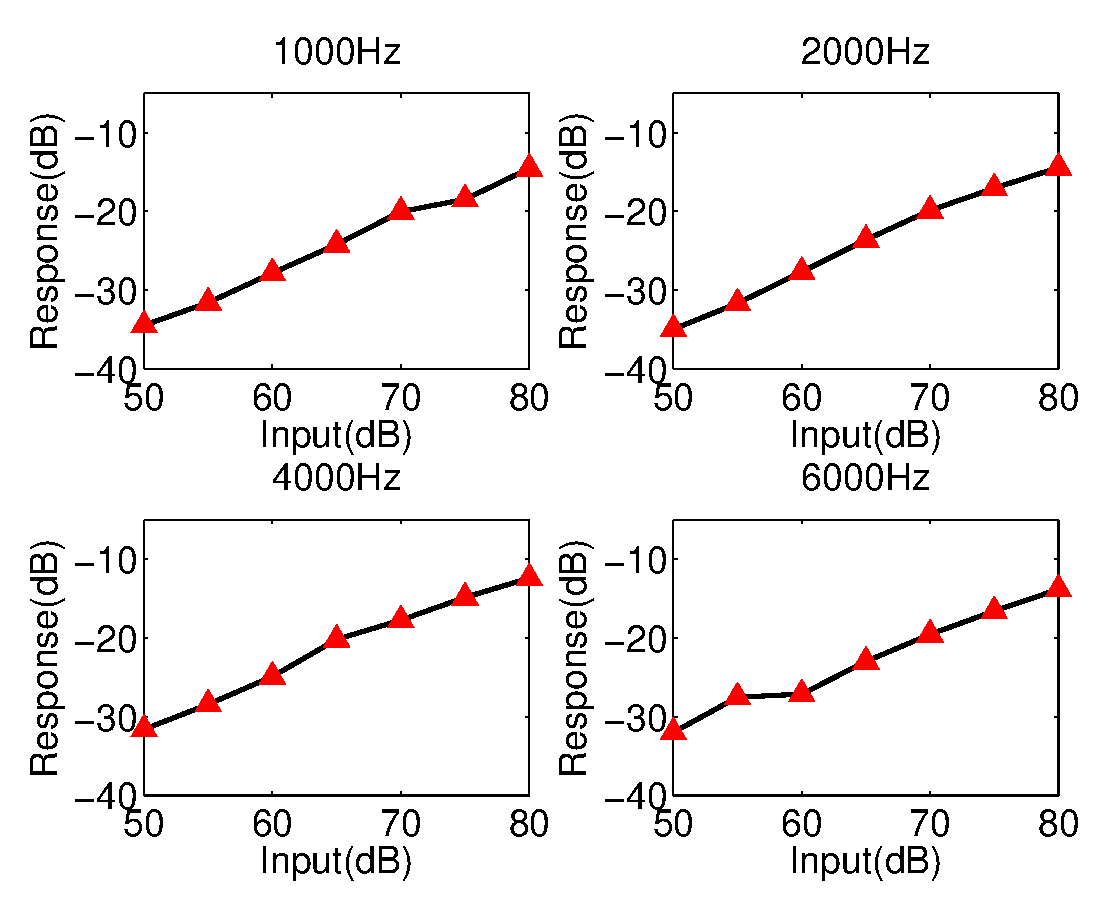
\includegraphics[scale=0.4]{calibration/CC_1.eps}
\caption{Frequency Response for Phone 1}
\label{fig:calibration_phone1}
\end{center}
\end{figure} 
\subsubsection{Directionality}